
\section{Product Backlog}
\label{sec:backlog}
In der folgenden Tabelle sind sämtliche Mindestanforderungen aufgeführt.
Sie beinhalten jeweils die Vorgangsnummer, den Namen, die Beschreibung und den Status der Anforderungen.
\begin{table}[H]
    \caption{Backlog}
    \centering
    \begin{tabularx}{\linewidth}{|c|X|X|c|}
        \hline
        \textbf{Vorgangs Nr.} & \textbf{Name} & \textbf{Beschreibung} & \textbf{Status} \\ \hline
        1 & Backend aufsetzen & Das Backend mithilfe von Spring initialisieren & fertig \\ \hline
        2 & Security Schnittstelle implementieren & Ermöglicht das sichere Einloggen und Registrieren & fertig \\ \hline
        3 & Schnittstelle für die Registrierung anlegen & Erstellung der Schnittstelle mit Spring & fertig \\ \hline
        4 & Schnittstelle für die Änderung der Nutzerdaten implementieren & Erstellung der Schnittstelle mit Spring & fertig \\ \hline
        5 & Schnittstelle für Login implementieren & Erstellung der Schnittstelle mit Spring & fertig \\ \hline
        6 & Schnittstelle für Logout implementieren & Erstellung der Schnittstelle mit Spring & fertig \\ \hline
        7 & Schnittstelle für die Erstellung einer Reservierung erstellen & Erstellung der Schnittstelle mit Spring & fertig \\ \hline
        8 & Schnittstelle zum Erhalten der eigenen Reservierungen implementieren & Erstellung der Schnittstelle mit Spring & fertig \\ \hline
        9 & Schnittstelle zum Löschen einer Reservierung implementieren & Erstellung der Schnittstelle mit Spring & fertig \\ \hline
        10 & Erstellung einer Homepage & Implementierung einer Startseite mit Informationen über die Car-Sharing Anwendung & fertig \\ \hline
        11 & Erstellung eines Login Buttons & Erstellung des Login Buttons und das Ansprechen der entsprechenden Schnittstelle & fertig \\ \hline
        12 & Erstellung eines Registrierungsbuttons & Platzierung des Buttons auf der Homepage und Öffnen eines Formulars & fertig \\ \hline
        13 & Erstellung der Registrierungsformulare & Erstellung der Formulare und Ansprechen der entsprechenden Schnittstelle mit den eingegebenen Werten & fertig \\ \hline
    \end{tabularx}
    \label{tab:backlog}
\end{table}
\newpage

\section{Beschreibung der ausgewählten Technologien und Werkzeuge}
\label{sec:technologien_wekzeuge}
Die im Folgenden aufgelisteten Technologien und Werkzeuge, inklusive Beschreibung, finden in dem Fastlane-Projekt Anwendung. \\

\textbf{IntelliJIDEA-IDE} ist eine integrierte Entwicklungsumgebung (IDE), die speziell für die Java-Entwicklung konzipiert ist.
Es ist eine leistungsstarke und weit verbreitete IDE, die Funktionen und Tools bietet, um den Entwicklungsprozess effizienter und produktiver zu gestalten.
IntelliJIDEA wurde von uns sowohl für das Backend, als auch das Frontend verwendet.\\

\textbf{Android Studio} ist eine integrierte Entwicklungsumgebung, die speziell für die Entwicklung von Android-Apps entwickelt wurde.
Es basiert auf der IntelliJ IDEA-Plattform und bietet umfangreiche Funktionen und Tools, um den gesamten Entwicklungsprozess für Android-Anwendungen zu unterstützen.
Da wir Fastlane Plattformunabhängig entwickeln, soll dieses auch auf Android-Tablets und Smartphones laufen.
Diesbezüglich fungiert Android Studio als Entwicklungsumgebung mit den notwendigen Tools.\\

\textbf{Visual Studio Code} ist ein plattformübergreifender, quelloffener Code-Editor.
Es ist eine leichte IDE mit etwaigen Funktionen, die die Entwicklung und Bearbeitung von Code in verschiedenen Programmiersprachen unterstützen.
Konkret wurde Visual Studio Code mit der \enquote{REST CLient} Erweiterung verwendet, um die REST-Schnittstellen des Backends zu testen.\\

\textbf{Java} ist eine objektorientierte Programmiersprache und findet Anwendung im Backend.
Sie zeichnet sich unter anderem durch Plattformunabhängigkeit, Zuverlässigkeit,
Robustheit und Sicherheit aus.
Zudem ist Java eine der meistverbreiteten Programmiersprachen der Welt und damit zukunftssicher, weshalb sich diese für dieses Projekt anbietet.\\

\textbf{Apache Maven} ist ein in der Programmiersprache Java geschriebenes Kommandozeilenwerkzeug aus der Kategorie
der Build-Werkzeuge.
Maven erleichtert uns durch Dependencies das Einbinden von Bibliotheken.
Die Dependencies werden in der pom.xml-Datei des Projektes aufgeführt.\\

\textbf{Spring} ist ein umfangreiches Java-Framework für die Entwicklung von Enterprise-Anwendungen.
Unter Enterprise-Anwendungen versteht man komplexe Softwarelösungen, welche der Automatisierung und Integration von Geschäftsprozessen und Datenverwaltung dienen.
Konkret in diesem Projekt wird Spring verwendet, um die REST-API bereit zustellen.
Darüber hinaus bietet das Spring-Framework etwaige Module und Erweiterungen, die für spezifische Anwendungsfälle wie Spring Security und Spring Boot entwickelt wurden.\\

\textbf{Spring Boot} ist ein Framework, das auf dem Spring-Framework aufbaut.
Durch diese Lösung wird der Aufwand, der von uns für die Konfiguration und Bereitstellung von Spring-Anwendungen aufgebracht werden muss, deutlich reduziert.\\

\textbf{Spring Security} ist ein leistungsstarkes Sicherheitsframework für Java-basierte Anwendungen, das entwickelt wurde,
um die Implementierung von Authentifizierung, Autorisierung und anderen Sicherheitsfunktionen zu vereinfachen.
Es integriert sich nahtlos mit dem Spring-Framework und bietet umfassende Funktionen zur Sicherung von Anwendungen.\\

\textbf{JSON} (JavaScript Object Notation) ist ein leichtgewichtiges Datenformat, das zur strukturierten Darstellung von Daten verwendet wird.
Es basiert auf der Syntax von JavaScript, ist jedoch unabhängig von einer bestimmten Programmiersprache.
In diesem Projekt wird ein \enquote{REST (Representational State Transfer)-API (Application Programming Interface)} verwendet,
wobei das Frontend mit dem Backend über REST-Schnittstellen kommuniziert.
JSON wird als Zwischenformat verwendet, um unter anderem Nutzerdaten zwischen den beiden Systemen, bzw. Programmiersprachen zu konvertieren.\\

\textbf{fasterxml/Jackson} ist eine leistungsstarke und weit verbreitete Java-Bibliothek zur Verarbeitung von JSON-Daten.
Es ermöglicht das Lesen, Schreiben und Manipulieren von JSON in Java-Objekte und umgekehrt.\\

\textbf{Dart} ist eine Programmiersprache, zur Entwicklung von plattformübergreifenden Anwendungen.
Sie ist die Basis für das Flutter-Framework.\\

\textbf{Flutter} ist ein Open-Source-Framework, das zur Erstellung plattformübergreifender, mobiler Anwendungen entwickelt wurde.
Mit Flutter ist es möglich native Benutzeroberflächen für iOS, Android, Windows und Web-Anwendungen aus einer einzigen Codebasis zu erstellen.
Mit Flutter wurde von uns das Frontend aufgesetzt. \\

\textbf{SQLite} wird von der Anwendung als eingebettete Datenbank verwendet.
Sie zeichnet sich durch Einfachheit, Portabilität und Geschwindigkeit aus.\\

\textbf{JUnit} ist ein Open-Source-Testframework, das von uns für Annotationen verwendet wurde.\\

\textbf{Lombok} ist eine Java-Bibliothek, die die Entwicklung der Java-Anwendung erleichtert, indem sie den Code für wiederkehrende Aufgaben reduziert.
Sie bietet Annotationen, die zur Generierung von Standardcode verwendet werden können. \\

\textbf{RESTAssured} haben wir für unsere Integrationstests genutzt.
Es ermöglicht uns, HTTP-Anfragen zu Testzwecken an die API zu senden und die entsprechenden Antworten zu überprüfen.\\

\textbf{nginx} ist ein leistungsstarker, Open-Source-Webserver und Reverse-Proxy-Server, der auch als Load Balancer, HTTP-Cache und Mail-Proxy eingesetzt werden kann.\\

\textbf{Confluence} ist eine kollaborative Plattform für das Team- und Projektmanagement.
Es ist eine Wiki-Software, die es dem Team und dem Kunden ermöglicht, gemeinsam an Inhalten zu arbeiten, Informationen zu teilen und Wissen rund um Fastlane zu dokumentieren.\\

\textbf{Jira} ist eine Projektmanagement-Software zur Verwaltung von Aufgaben, Projekten und Arbeitsabläufen.
Die Anforderungen, die wir bei Confluence gemeinsam mit dem Kunden festgelegt haben, wurden in Jira als Tasks überführt und konnten so unabhängig und systematisch von Teammitgliedern abgearbeitet werden.\\

\newpage

\textbf{Bitbucket} ist eine webbasierte Plattform für die Versionsverwaltung von Quellcode und die Zusammenarbeit an dem Softwareprojekt.
Es bietet Funktionen für das Hosting vom Git-Repository, die Verfolgung von Änderungen, Pull-Requests, Code-Reviews und die Integration mit anderen Entwicklungstools.
Bearbeitet ein Teammitglied einen Task von Jira, so wurde dafür ein Branch auf Bitbucket erstellt in dem unabhängig vom restlichen Projekt gearbeitet werden konnte.
Dies vermeidet größere Fehler, durch beispielsweise Merge-Konflikte auf dem Master.\\

\textbf{Git-Repository} ist ein Speicherort, in dem Git die Versionshistorie und den Quellcode eines Projekts speichert.
Es enthält alle Dateien der Fastlane-Anwendung und Ordner und Informationen, die für die Versionsverwaltung mit Git benötigt werden.\\

\textbf{Docker} ist eine Open-Source-Plattform, um Anwendungen in Containern zu isolieren und bereitzustellen.
Mithilfe von Docker können wir die Anwendung und ihre Abhängigkeiten in standardisierte Container verpacken, die dadurch unabhängig von der zugrunde liegenden Infrastruktur lauffähig ist.\\

\textbf{Docker Compose}  ist ein Tool, das die Verwaltung und Orchestrierung von mehreren Docker-Containern ermöglicht.
Mit Docker Compose können wir eine Anwendung in einer einzigen Konfigurationsdatei beschreiben, die als \enquote{docker-compose.yml} zu finden ist.
Diese Datei definiert die Container, ihre Konfigurationen, Netzwerke und Abhängigkeiten.\\

\textbf{Docker Desktop} ist eine Softwareanwendung, die die Verwendung von Docker auf Desktop-Computern ermöglicht.
Es handelt sich um eine Benutzeroberfläche und ein Toolset, das Docker-Container auf lokalen Maschinen einrichten, verwalten und ausführen kann.
In Docker Desktop sind alle vorhandenen Container einer Maschine aufgelistet, was uns während der Entwicklung eine bessere Übersicht und Verwaltung aller Container ermöglicht.\\

\textbf{Figma} ist ein browserbasiertes Design- und Prototyping-Tool.
Es ermöglicht das zusammenzuarbeiten in Echtzeit, Designs zu erstellen, zu bearbeiten und zu teilen.
Über Figma wurden erste Designideen für das Frontend entwickelt und festgehalten.
Sobald wir mit einem Design zufrieden waren, wurde dieses beispielsweise durch Widgets im Frontend umgesetzt.\\

\textbf{Materialdesign} ist ein Designkonzept für die Gestaltung von Benutzeroberflächen in Apps und Websites.
Es bietet eine kohärente Designsprache und eine umfassende Designrichtlinie für die Entwicklung von Apps und Websites.
Materialdesign wurde von uns, neben Figma für das Design des Frontends verwendet.
Jedoch wurde weitestgehend mit Figma gearbeitet. \\

\textbf{Visual Paradigm} ist eine umfassende Software-Suite für das Modellieren und die Entwicklung von Softwarelösungen.
In Zusammenhang mit dem Fastlane-Projekt stellt dieses Tools und Funktionen für die UML-Modellierung zur Verfügung.\\

\newpage

\section{Beschreibung der git Repository Struktur}
\label{sec:git}
Das Entwicklerteam nutzt Atlassian-Produkte, darunter Confluence und Jira, und hat sich daher für Bitbucket als Versionsverwaltung entschieden.
Die Entscheidung basiert auf den Vorteilen, dass erstellte Aufgaben über Jira direkt als Branches in Bitbucket erstellt werden können.
Dies optimiert die Projektverwaltung und Planung, was zu Zeitersparnis und gesteigerter Effizienz führt.
Bitbucket fungiert ausschließlich als Hosting-Plattform für Git-Repositories.
Die Entwickler arbeiten dabei mit sogenannten Branches im Git-Repository.
Wurde ein Branch auf Bitbucket erstellt, so konnte von diesem lokal eine Kopie angelegt werden, um Änderungen zu speichern und anschließend in das Git-Repository hochzuladen.
Für jeden erstellten Task in Jira wurde auf Bitbucket ein eigener Feature-Branch erstellt.
Dadurch wird ermöglicht, dass die Aufgaben unabhängig voneinander bearbeitet werden können und das Risiko schwerwiegender Fehler, beispielsweise durch Merge-Konflikte auf dem Master-Branch, verringert wird.

Um einen Merge auf den Master-Branch durchzuführen, war es erforderlich, einen Merge-Request im jeweiligen Feature-Branch zu erstellen.
Auf dem Master-Branch wurden ausschließlich funktionierende Features gepusht und zusammengeführt.
Dadurch wurde sichergestellt, dass nur vollständig getestete und funktionsfähige Änderungen im Master-Branch vorhanden sind.\\

Das Repository ist in den Sektionen \textbf{code} und \textbf{doku} unterteilt.
Diese Aufteilung ermöglicht eine strukturierte Verwaltung der Projektressourcen und eine klare Trennung zwischen der Dokumentation und dem eigentlichen Code.
Dadurch wird die Zusammenarbeit und Entwicklung erleichtert.
In der Sektion \enquote{doku} befinden sich die bearbeiteten Laboraufgaben.
Die Sektion \enquote{code} ist unterteilt in frontend und backend.  \\
Für das \enquote{Frontend} wurde \enquote{Flutter} verwendet, diesbezüglich gibt es Unterordner für verschiedene Plattformen, wie Ios, Android und windows.
In dem Ordner \enquote{lib} befinden sich alle relevanten Dateien und Ordner für die Entwicklung der Benutzeroberfläche.
Die Aufteilung erfolgt in die Ordner \enquote{Constants}, \enquote{control}, \enquote{data}, \enquote{model}, \enquote{widgets} und der Main-Datei \enquote{mainDashboard}.    \\
Die Sektion \enquote{bakend} enthält einen Ordner \enquote{Entwurf} in dem alle Entwürfe hinterlegt sind und den Ordner \enquote{fastlane}
in dem alle Dateien und Ordner für die Entwicklung der serverseitigen Logik vorhanden sind.
Die wichtigsten Daten in diesem Ornder sind die Datenbank, ein Dockerfile, ein Ordner namens \enquote{requests} zum Testen der Schnittstellen und der Source-Ordner \enquote{src}.
Im Source-Ornder befindet sich neben dem Main-Ornder ein Test-Ordner, in dem unter anderem alle Kontroller getestet werden.
Der Main-Ordner enthält die ausführbare Datei \enquote{FastlaneApplication} sowie Ordner, die alle Funktionen und Daten für das Backend beinhalten.






\section{Architekturbeschreibung für das Gesamtsystem}
\label{sec:architektur}
\input{content/4/4_architekturbeschreibung}

    \subsection{Komponentendiagramm}
    \label{subsec:komponentendiagramm}
    \begin{figure}[H]
    \centering
    \includegraphics[width = \textwidth]{pictures/fastlane_komponentendiagramm}
    \caption{Komponentendiagramm}
    \label{fig:komponentendiagramm}
\end{figure}
\clearpage
Das Gesamtsystem kann in drei Packages unterteilt werden, um eine bessere Übersicht zu gewährleisten:
\begin{enumerate}
    \item Das Frontend wurde mit Flutter erstellt und umfasst die Web-Anwendung, die Desktop-App und die Mobile-App.
    Diese können über HTTP-Anfragen mit dem Backend kommunizieren.
    \item Das Backend wurde mithilfe von Java und dem Spring Framework entwickelt.
    Es ist in drei kleinere Packages unterteilt:
    \begin{itemize}
        \item Control: Hier befinden sich die Schnittstellendefinitionen für die HTTP-Anfragen.
        Die Controller rufen entsprechende Methoden in den Services auf, um die eingehenden Anfragen zu verarbeiten.
        \item Service: Die Services validieren die Anfragen und können bei Bedarf über die JPA Repositories
        auf die Datenbank zugreifen, um die erforderliche Logik umzusetzen.
        \item JPA Repository: Diese Repositories dienen als Interfaces für den Zugriff auf die SQLite Datenbank.
        Sie sind direkt mit der Datenbank verbunden und ermöglichen das Speichern, Abrufen und Bearbeiten von Daten.
    \end{itemize}
    \item Die Datenbank, welche unter SQLite läuft.
\end{enumerate}

Zusätzlich werden die Verbindungen zwischen den Services dargestellt, da diese auch untereinander kommunizieren.
Beispielsweise ist der \enquote{RegistrationService} mit dem \enquote{AccountService} verbunden, da bei der
Registrierung ein Account erstellt werden muss.

    \subsection{Modellierung der statischen und dynamischen Sicht}
    \label{subsec:statische_und_dynamische_sicht}
    \subsubsection{Entity-Relationship-Diagramm}
\begin{figure} [H]
    \centering
    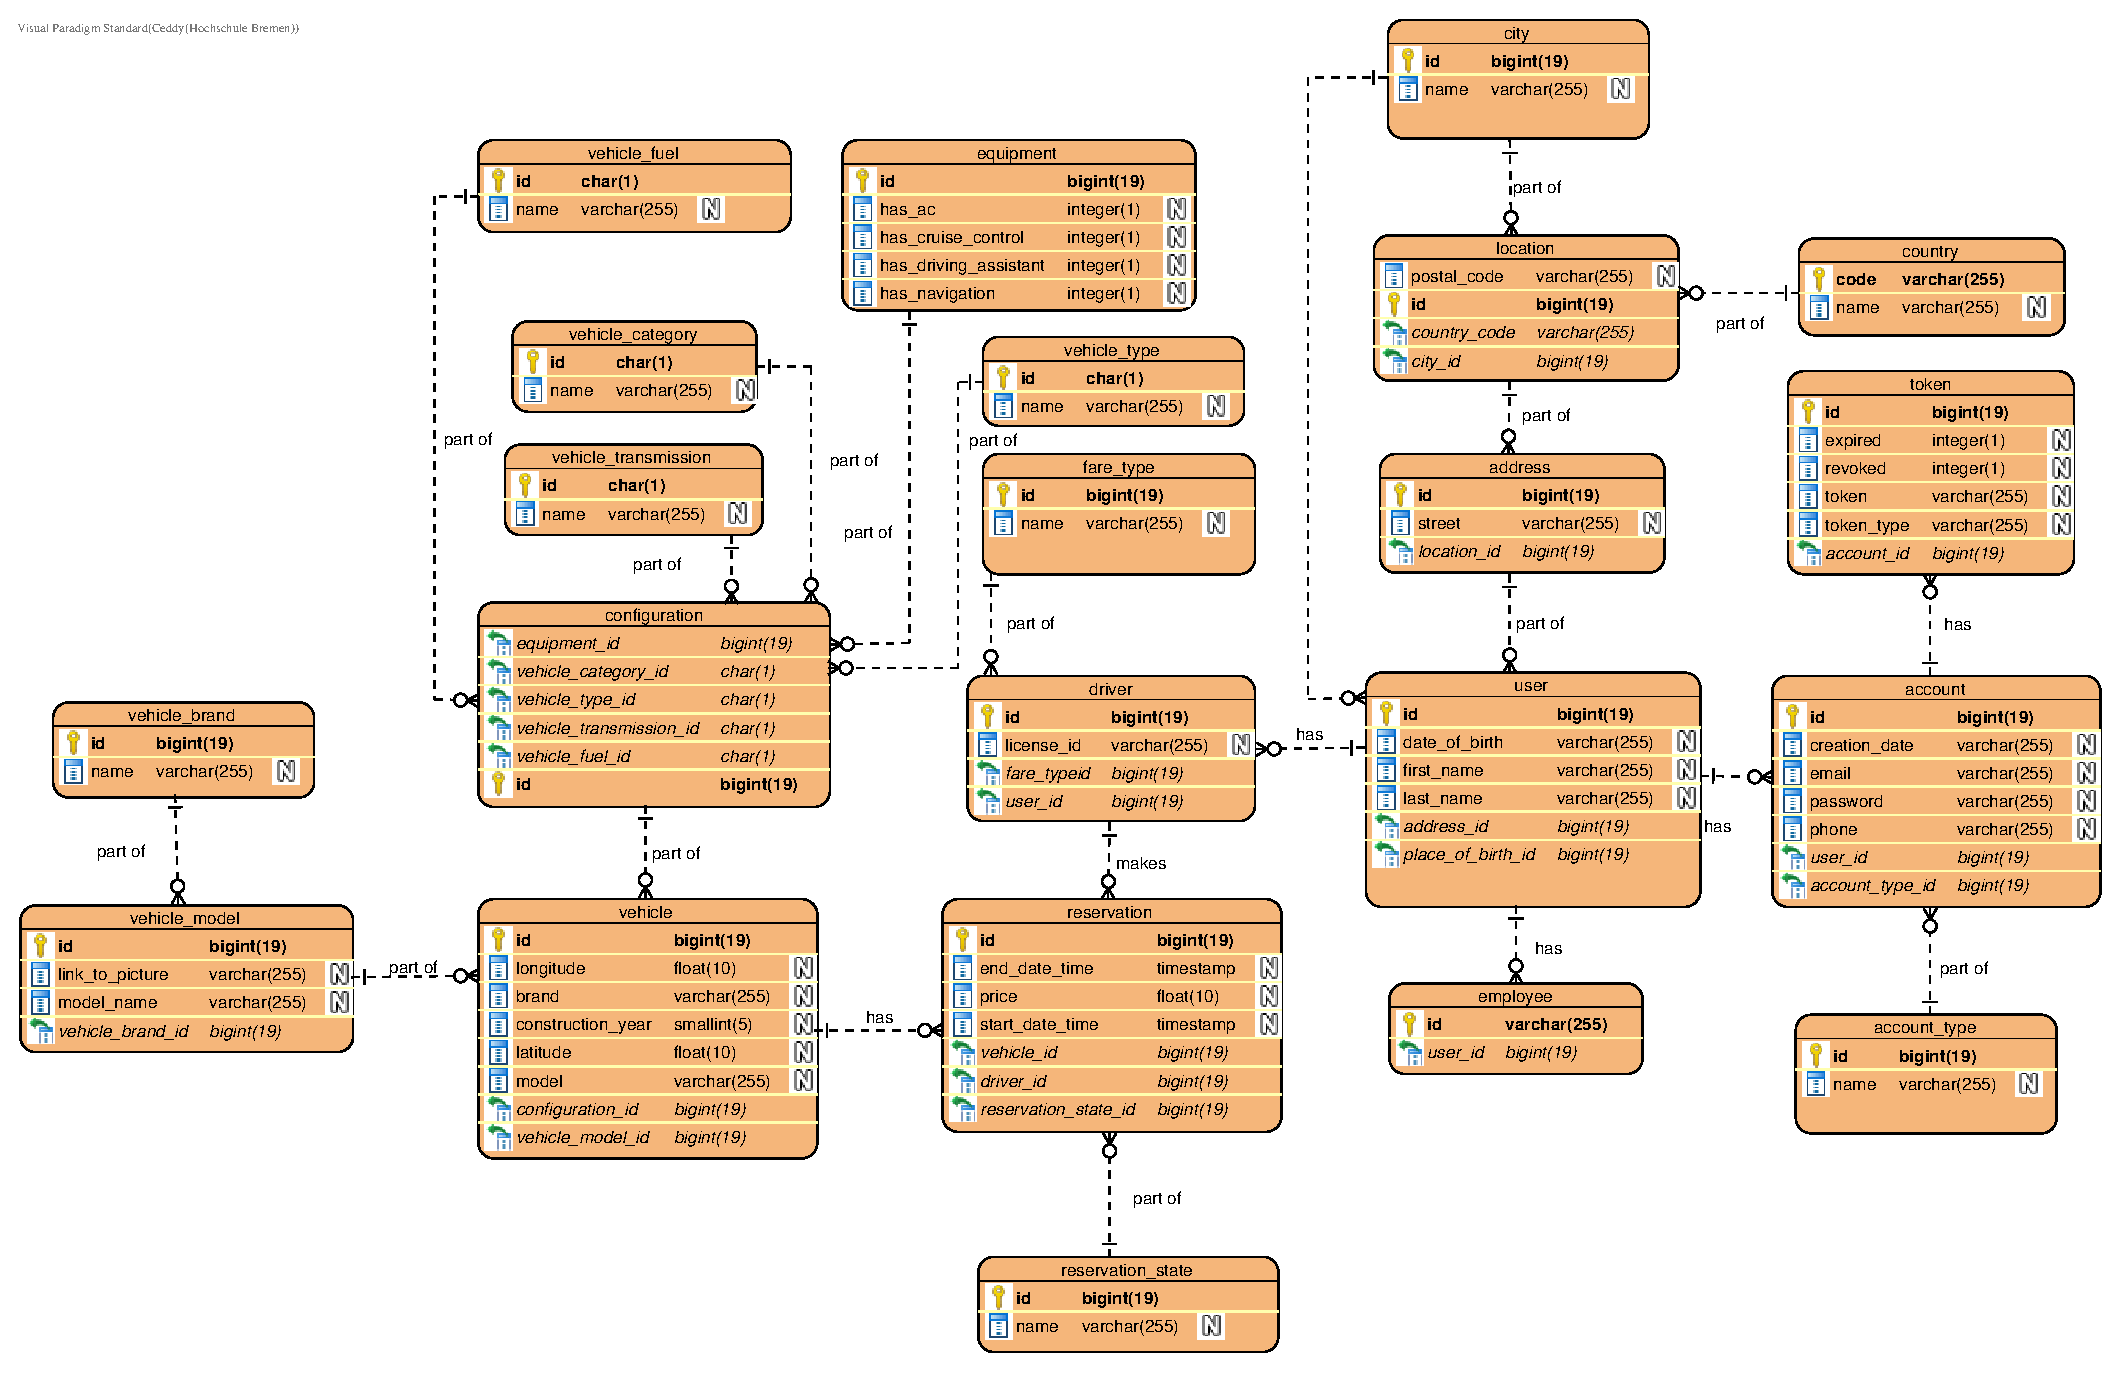
\includegraphics[width=1\textwidth]{pictures/Fastlane-ERD}
    \caption{Entity-Relationship-Diagramm}
    \label{fig:ERD}
\end{figure}

\bigskip

Das ER-Diagramm stellt die Entitäten und deren Relationen in der Datenbank des Systems dar.
Sowohl ein \enquote{Employee} als auch ein \enquote{Driver} können auf dieselbe natürliche Person verweisen.
Dies ermöglicht es, dass eine Person sowohl als Angestellter als auch als Fahrer agieren kann, je nach den Anforderungen und Rollen in diesem System.
Durch diese flexible Gestaltung kann gewährleistet werden, dass die Benutzer verschiedene Rollen und Funktionen zugewiesen können, ohne dass separate Benutzerinstanzen erstellt werden müssen.
Außerdem befindet sich die Datenbank in der dritten Normalform, was eine strukturierte und optimierte Speicherung der Daten gewährleistet.
Durch die Verwendung zentraler Entitäten und die Vermeidung unnötiger Dubletten können Änderungen effizient an einer einzigen Stelle vorgenommen werden, was die Wartung und Verwaltung erleichtert und potenzielle Inkonsistenzen minimiert.

\bigskip

\subsubsection{Deployment-Diagramm}

\begin{figure} [H]
    \centering
    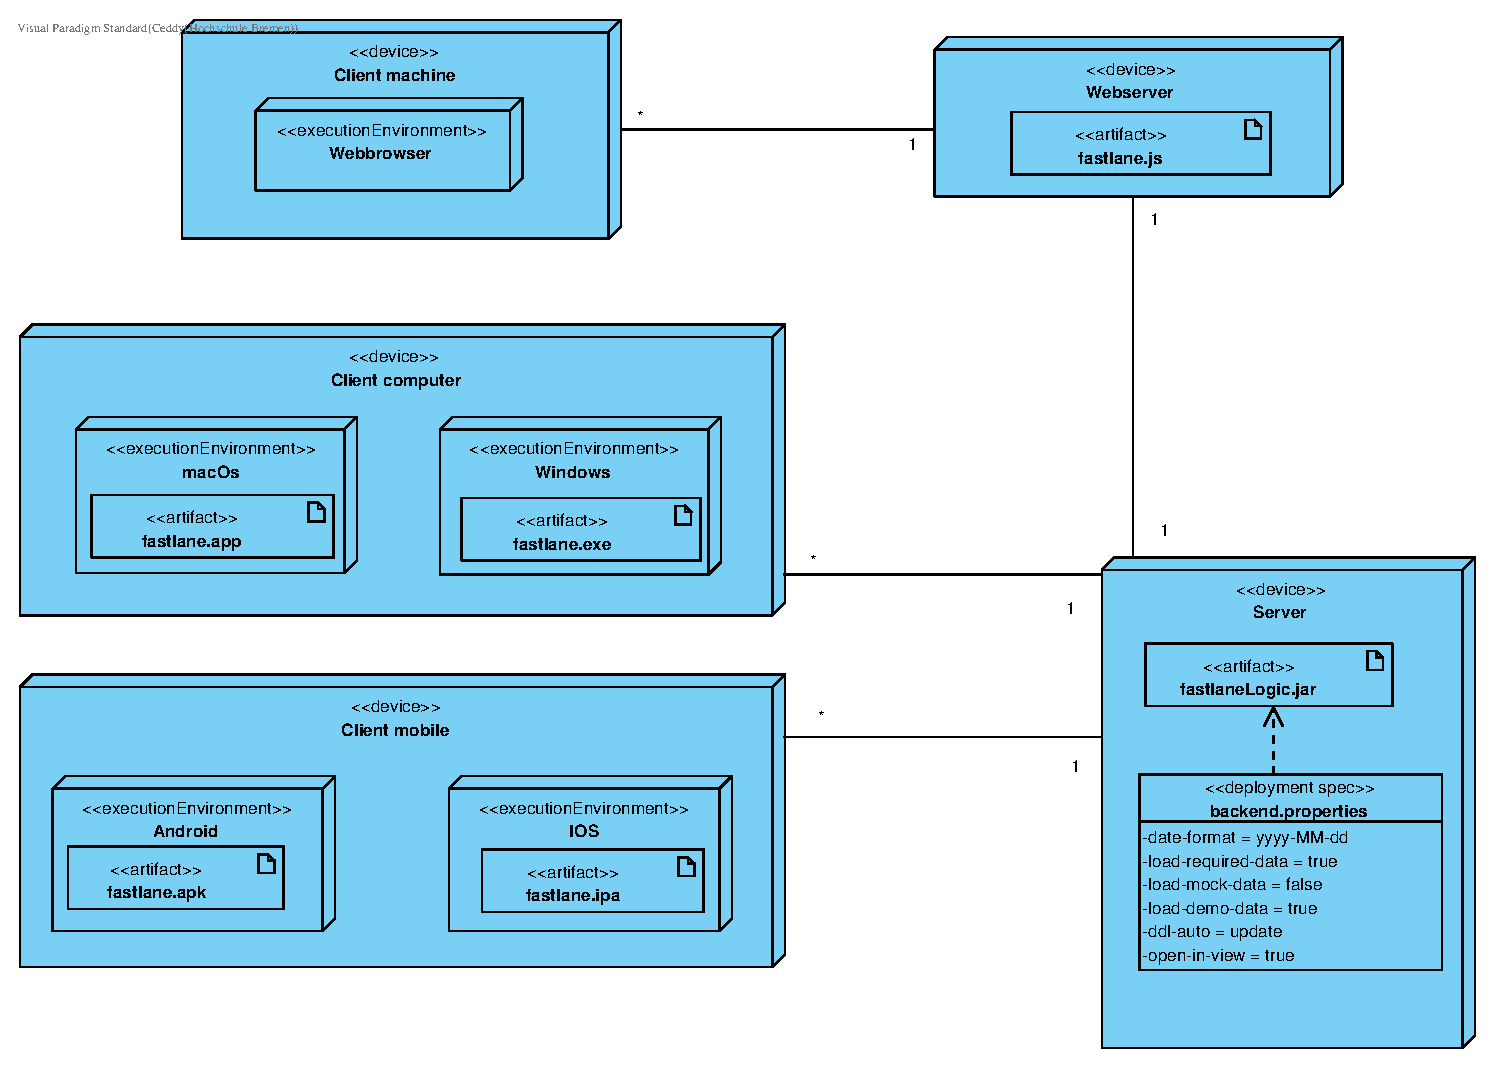
\includegraphics[width=1\textwidth]{pictures/Fastlane_Deployment_Diagram}
    \caption{Deployment-Diagramm}
    \label{fig:Deployment-Diagram}
\end{figure}

\bigskip


Das folgende Diagramm zeigt die Verteilung des Systems auf die verschiedenen Geräte und Ausführungsumgebungen.
Die Flexibilität von Flutter ermöglicht es, die Frontend-Anwendungen in verschiedenen Ausführungsumgebungen auszuführen, was eine entsprechende Verteilung erforderlich macht.
Die Backend-Anwendung wird auf einem dedizierten Server ausgeführt und stellt die Kernfunktionalität und Datenverarbeitung bereit.
Um die Daten für den Webbrowser auf beliebigen Geräten bereitzustellen, wird ein Webserver verwendet, der die Daten per HTTPS liefert.
In diesem Deployment-Diagramm wurde der Webbrowser auf einem Client-Device platziert, um die Ausführungsumgebung nicht doppelt auf dem Client-Computer und dem Client-Mobilgerät darstellen zu müssen.
Die ausführbaren Dateien, die das Frontend enthalten, werden in den Ausführungsumgebungen der jeweiligen Geräte ausgeführt.
Ein beispielhaftes Szenario zeigt die Ausführung der fastlane.apk auf einem Android-Gerät, das in der entsprechenden Umgebung auf einem Client-Mobilgerät läuft.
Durch diese Verteilung der Komponenten auf die Geräte und Ausführungsumgebungen kann die Software plattformübergreifend genutzt werden, wobei jedes Gerät die spezifischen Anforderungen der jeweiligen Ausführungsumgebung erfüllen muss.

\bigskip

\subsubsection{Sequenz-Diagramm}
\begin{figure}[H]
    \centering
    \includegraphics[width = 0.87\textwidth]{pictures/fastlane_sequenz_diagramm}
    \caption{Sequenzdiagramm}
    \label{fig:sequenzdiagramm}
\end{figure}

Das abgebildete Sequenzdiagramm stellt den Vorgang des Registrierens dar.
Dabei ist zu beachten, dass die Requests an die entsprechende Serveradresse gesendet werden.
Somit würde beispielsweise ein vollständiger Request an die localhost Adresse, über den Port 8080 folgendermaßen
aussehen: http://localhost:8080/driver/exist/licenseId.
Zu Beginn der Registrierung muss der Nutzer seine Führerschein Id eingeben.
Daher wird ein HTTP-Request an das Backend an den Endpunkt \enquote{/driver/exist/licenseId} gesendet.
Existiert die Führerschein Id noch nicht, so wird der Status Code 200 Ok zurückgesendet.
Ist die Id allerdings schon im System vorhanden, wir der Status Code 409 Conflict
zurückgesendet. \medskip

Zu einem späteren Zeitpunkt der Registrierung wird vom Benutzer eine E-Mail eingegeben.
Dabei läuft der gleiche Prozess erneut ab.
Es wird ein HTTP-Request an den Endpunkt \enquote{account/exist/email} gesendet.
Wenn die E-Mail bereits im System existiert, wird der Status Code 409 Conflict zurückgesendet.
Existiert sie allerdings noch nicht, wird der Status Code 200 Ok gesendet. \medskip

Sobald der Nutzer mit der Eingabe seiner Daten fertig ist, wird ein Post Request an den
Endpunkt \enquote{/register/member} gesendet.
Dabei werden im Body des Requests alle eingegebenen Daten mitgegeben.
Sofern die Registrierung im Backend erfolgreich verläuft, wird der Status Code 201 Created gesendet.
Tritt jedoch ein Fehler auf, wird der Status Code 401 Unauthorized zurückgesendet. \medskip

Dieses Diagramm stellt nur die Registrierung dar, allerdings laufen die meisten Prozesse nach dem gleichen Prinzip
ab.
Sobald im Frontend ein Request gesendet wird, wird dieser im Backend verarbeitet und der Entsprechende Status Code
mit dem Passenden Body zurückgesendet.

\section{Beschreibung der implementierten Komponenten/Module}
\label{sec:implementierte_komponenten}
Es wurden verschiedene Schnittstellen erstellt, um die Kommunikation mit dem Backend zu ermöglichen.
Jede Schnittstelle bietet eine spezifische Funktion.
Einige Schnittstellen werden in der aktuellen Version noch nicht von dem Frontend genutzt.
Somit bietet das Backend einiges mehr an Funktionalität, welche in den kommenden Versionen von dem Frontend
aufgegriffen wird.
Um unbefugten Zugriff auf diese Schnittstellen zu verhindern,
wurden Zugriffsrechte basierend auf den Rollen der Benutzer festgelegt.
Die folgende Tabelle gibt einen Überblick über alle Schnittstellen und die Zugriffsrechte für die verschiedenen Rollen.
Das \checkmark Symbol steht für vollen Zugriff,
das \textcircled{} Symbol für Zugriff auf eigene Ressourcen des Nutzers und keine Markierung bedeutet keinen Zugriff.
Die Rollen werden durch die Abkürzungen \enquote{A} für Admin,
\enquote{M} für Mitarbeiter und \enquote{K} für Kunde dargestellt.

\begin{xltabular}{\textwidth}{|l|l|X|c|c|c|}
    \caption{Implementierte Schnittstellen} \label{tab:schnittpunkte}\\
    \hline
    \textbf{Methode} & \textbf{Endpunkt} & \textbf{Beschreibung} & \textbf{A} & \textbf{M} & \textbf{K} \\
    \hline
    \endfirsthead
    \caption[]{Fortsetzung \enquote{Implementierte Schnittstellen}} \\
    \hline
    \textbf{Methode} & \textbf{Endpunkt} & \textbf{Beschreibung} & \textbf{A} & \textbf{M} & \textbf{K} \\
    \hline
    \endhead
    \hline \multicolumn{6}{r}{$\hookrightarrow$} \\
    \endfoot
    \hline
    \endlastfoot
    \hline
    \multicolumn{6}{|l|}{\textbf{Account}} \\
    \hline
    GET & /account & Liefert alle Accounts. & $\checkmark$ & $\checkmark$ & \\
    \hline
    GET & /account/id/\{id\} & Liefert Account anhand der Id. & $\checkmark$ & $\checkmark$ & $\bigcirc$ \\
    \hline
    GET & /account/email/\{email\} & Liefert Account anhand der Email. & $\checkmark$ & $\checkmark$ & \\
    \hline
    GET & /account/exist/\{email\} & Überprüft, ob unter der Email bereits ein Account existiert. & $\checkmark$ & $\checkmark$ & $\checkmark$ \\
    \hline
    PATCH & /account/\{email\}/\{id\} & Erneuert den Account mit den übergebenen Werten. & $\checkmark$ & $\checkmark$ & $\bigcirc$ \\
    \hline
    DELETE & /account/\{id\} & Löscht den Account mit der angegebenen Id. & $\checkmark$ & $\checkmark$ & $\bigcirc$ \\
    \hline
    \multicolumn{6}{|l|}{\textbf{Authentication}} \\
    \hline
    POST & /auth/login & Loggt den übergebenen Nutzer ein und liefert die Authentisierung. & $\checkmark$ & $\checkmark$ & $\checkmark$ \\
    \hline
    \multicolumn{6}{|l|}{\textbf{Driver}} \\
    \hline
    GET & /driver/exist/\{licenseId\} & Überprüft, ob bereits ein Mitgliedskonto mit dieser Führerscheinnummer existiert. & $\checkmark$ & $\checkmark$ & $\checkmark$ \\
    \hline
    GET & /driver/user/\{userId\}/\{accountId\} & Liefert den Driver anhand der UserId. & $\checkmark$ & $\checkmark$ & $\bigcirc$ \\
    \hline
    PATCH & /driver/\{id\}/\{accountId\} & Erneuert den Driver mit den übergebenen Werten. & $\checkmark$ & $\checkmark$ & $\bigcirc$ \\
    \hline
    \multicolumn{6}{|l|}{\textbf{Employee}} \\
    \hline
    GET & /employee & Liefert alle Employees. & $\checkmark$ & & \\
    \hline
    GET & /employee/\{id\} & Liefert Employee anhand der Id. & $\checkmark$ & & \\
    \hline
    \multicolumn{6}{|l|}{\textbf{Health}} \\
    \hline
    GET & /health/ping & Liefert die aktuelle Zeit des Servers zurück. & $\checkmark$ & $\checkmark$ & $\checkmark$ \\
    \hline
    GET & /health/database & Überprüft den Status der Datenbank und liefert diesen zurück. & $\checkmark$ & $\checkmark$ & $\checkmark$ \\
    \hline
    \multicolumn{6}{|l|}{\textbf{Registration}} \\
    \hline
    POST & /register/member & Ermöglicht die Registrierung eines Kunden. & $\checkmark$ & $\checkmark$ & $\checkmark$ \\
    \hline
    POST & /register/employee & Ermöglicht die Registrierung eines Mitarbeiters. & $\checkmark$ & & \\
    \hline
    \multicolumn{6}{|l|}{\textbf{Reservation}} \\
    \hline
    GET & /reservation & Liefert alle Reservations. & $\checkmark$ & $\checkmark$ & $\checkmark$ \\
    \hline
    GET & /reservation/\{id\} & Liefert die Reservation anhand der Id. & $\checkmark$ & $\checkmark$ & $\checkmark$ \\
    \hline
    GET & /reservation/driver/\{driverId\} & Liefert alle Reservations des angegebenen Fahrers. & $\checkmark$ & $\checkmark$ & $\checkmark$ \\
    \hline
    POST & /reservation & Erstellt eine neue Reservation. & $\checkmark$ & $\checkmark$ & $\checkmark$ \\
    \hline
    PATCH & /reservation/\{id\} & Erneuert die Reservation mit den übergebenen Werten. & $\checkmark$ & $\checkmark$ & $\checkmark$ \\
    \hline
    DELETE & /reservation/\{id\} & Löscht die Reservation mit der angegebenen Id. & $\checkmark$ & $\checkmark$ & $\checkmark$ \\
    \hline
    \multicolumn{6}{|l|}{\textbf{Vehicle}} \\
    \hline
    GET & /vehicle & Liefert alle Vehicles. & $\checkmark$ & $\checkmark$ & $\checkmark$ \\
    \hline
    GET & /vehicle/\{id\} & Liefert das Vehicle anhand der Id. & $\checkmark$ & $\checkmark$ & $\checkmark$ \\
    \hline
    GET & /vehicle/free & Liefert alle freien Vehicles. & $\checkmark$ & $\checkmark$ & $\checkmark$ \\
    \hline
    GET & /vehicle/reservation/\{reservationId\} & Liefert das Vehicle, welches für die angegebene Reservation reserviert ist. & $\checkmark$ & $\checkmark$ & $\checkmark$ \\
    \hline
    PATCH & /vehicle/\{id\} & Erneuert das Vehicle mit den übergebenen Werten. & $\checkmark$ & $\checkmark$ & $\checkmark$ \\
    \hline
    DELETE & /vehicle/\{id\} & Löscht das Vehicle mit der angegebenen Id. & $\checkmark$ & $\checkmark$ & $\checkmark$ \\
    \hline
\end{xltabular}

\section{Verifikation}
\label{sec:verifikation}
Bereits während der Entwurfsphase unserer Anwendung war eine grundlegende Frage präsent: Wie können wir sicherstellen, dass unser Produkt gemäß den Vorgaben funktioniert und alle Anforderungen erfüllt?
Die Lösung fanden wir in der Erstellung eines umfassenden Testkonzepts, das darauf abzielte, die folgenden Kernfragen zu beantworten:

\begin{itemize}
    \item Was testen wir?
    \item Welche Teststrategie wenden wir an?
    \item Wie testen wir?\ Was ist unser Workflow?
    \item Wie dokumentieren wir?
    \item Welche Werkzeuge nutzen wir?
    \item Benötigen wir Testdaten? Wenn ja, wie generieren wir solche?
\end{itemize}

    \subsection{Unser Testkonzept}
    \label{subsec:test_konzept}
    \textbf{Was testen wir?}\smallskip

Um sicherzustellen, dass alle vom Backend bereitgestellten Schnittstellen ordnungsgemäß funktionieren,
haben wir uns dazu entschlossen, alle Schnittstellen zu testen.
Zudem haben wir festgelegt, dass wir im Frontend die Mindestanforderungen testen.

\bigskip
\textbf{Welche Teststrategie wenden wir an?}\smallskip

Für die Backendtests haben wir uns für den ausschließlichen Einsatz von automatisierten Integrationstests entschieden.
Der Hauptgrund für diese Entscheidung ist, dass diese eine ausgewogene Balance zwischen Codeabdeckung und der Prüfung der korrekten Kommunikation zwischen den verschiedenen Schichten bieten.
Für komplexere Methoden (zum Beispiel einige Update-Methoden), die typischerweise durch Unit-Tests abgedeckt werden sollten, haben wir uns für einen Kompromiss entschieden.
Solche Methoden werden durch eine hinreichende Anzahl von Integrationstests, die auch Randfälle berücksichtigen, auf mögliche Fehlfunktionen hin untersucht.\medskip

Aufgrund zeitlicher Begrenzungen haben wir uns dazu entschlossen, die Funktionalität des Frontends ausschließlich durch manuelle Tests zu prüfen.

\bigskip
\textbf{Wie testen wir? Was ist unser Workflow?}\smallskip

Nach der Implementierung einer Schnittstelle haben wir diese unmittelbar getestet.
Hierfür haben wir Testszenarien nach der \enquote{Given-When-Then}-Methode entwickelt
und anschließend jedes Szenario in einzelne Tests aufgeteilt.
Bei jeder neuen Version wurden alle Tests ausgeführt.
Falls ein Test fehlschlug, konnte der Fehler aufgrund der atomaren Natur schnell lokalisiert und behoben werden. \medskip

Für die Testung des Frontends haben wir uns ebenfalls Szenarien nach der \enquote{Given-When-Then}-Methodik ausgedacht und diese im Nachhinein manuell durchgetestet.

\bigskip
\textbf{Wie dokumentieren wir?}\smallskip

Wie zuvor angeführt, ist es die Aufgabe jedes Entwicklers, nach der Umsetzung einer Schnittstelle Testfälle dafür zu erstellen.
Wir haben uns darauf verständigt, diese Testfälle sorgfältig zu protokollieren, um deren Nachvollziehbarkeit zu gewährleisten.
Dabei galt es, das folgende Schema zu befolgen: \bigskip

\resizebox{\textwidth}{!}{%
    \begin{tabular}{|l|cl|cl|cl|l|}
        \hline
        &
        \multicolumn{2}{c|}{Given} &
        \multicolumn{2}{c|}{When} &
        \multicolumn{2}{c|}{Then} &
        \\ \hline
        \multicolumn{1}{|c|}{Testnummer} &
        \multicolumn{1}{c|}{Beschreibung} &
        \multicolumn{1}{c|}{Rolle} &
        \multicolumn{1}{c|}{Request Method} &
        \multicolumn{1}{c|}{Endpunkt} &
        \multicolumn{1}{c|}{erwarteter   Statuscode} &
        \multicolumn{1}{c|}{erwartete   Ausgabe im Body} &
        \multicolumn{1}{c|}{OK?} \\ \hline
        &
        \multicolumn{1}{l|}{} &
        &
        \multicolumn{1}{l|}{} &
        &
        \multicolumn{1}{l|}{} &
        &
        \\ \hline
    \end{tabular}%
}

\bigskip
\textbf{Welche Werkzeuge nutzten wir zur Durchführung der Tests?}\smallskip

Für die Durchführung unserer automatisierten Tests haben wir eine Kombination aus verschiedenen Bibliotheken verwendet.
Einige dieser Bibliotheken sind bereits integraler Bestandteil von Spring Boot.
Spring Boot bietet außerdem die Möglichkeit, zu Testzwecken eine reduzierte Version der Anwendung unter einem anderen Port zu starten.
Zur Steuerung der Testreihenfolge haben wir Annotationen aus der \enquote{JUnit 5} Bibliothek verwendet.
Die Integrationstests wurden mithilfe der Bibliothek \enquote{RESTAssured} durchgeführt, welche alle erforderlichen Methoden zur Simulation von API-Anfragen nach der Methodik \enquote{Given-When-Then} bereitstellt.
Schließlich verwendeten wir Hamcrest, um die tatsächlichen Rückgabewerte mit den erwarteten Ergebnissen abzugleichen.

\bigskip
\textbf{Benötigen wir Testdaten? Wenn ja, wie generieren wir solche?}\smallskip

Einige unserer Tests, wie zum Beispiel das Löschen eines Accounts, setzen voraus, dass bereits Accounts in der Datenbank vorhanden sind.
Daher war es erforderlich, das Vorhandensein solcher Daten zu simulieren.
Hierfür haben wir den Dienst \enquote{Mockaroo} in Anspruch genommen.
\enquote{Mockaroo} ist ein Online-Tool, das entwickelt wurde, um realistische Testdaten in verschiedenen Formaten (wie CSV, JSON, SQL und Excel) zu generieren.
Vor der Durchführung des ersten Tests haben wir all diese Daten in die Datenbank eingepflegt, um eine adäquate Testumgebung zu schaffen.

    \subsection{Verification Matrix}
    \label{subsec:verification_matrix}
    Im Folgenden finden sie ein umfassende Tabelle, die alle entweder im Frontend oder im
Backend getesteten Anforderungen enthält.
Des Weiteren wird in den Spalten \enquote{Testnummer Backend} und \enquote{Testnummer Frontend} die Nummer
des jeweiligen Tests erfasst.
Die Nummern für die Backend Tests sind in \hyperref[subsec:testfaelle_backend]{Testfälle Backend} wiederzufinden.
Die Nummern der Frontend Tests sind in \hyperref[subsec:testfaelle_frontend]{Testfälle Frontend} zu finden.

\begin{longtable}{|m{2cm}|m{6.5cm}|m{2.5cm}|m{2.5cm}|}
    \hline
    \textbf{ID} & \textbf{Beschreibung} & \textbf{Testnummer Backend} & \textbf{Testnummer Frontend} \\
    \hline
    FA-5 & Mitgliedskonten dürfen nur angelegt werden, wenn die Person mindestens 18 Jahre alt ist & 2 & 2 \\
    \hline
    FA-6 & Die Anwendung soll über eine URL erreichbar sein & Durch alle Tests gewährleistet & - \\
    \hline
    FA-29 & Mitgliedskonten müssen durch einen Mitglied angelegt werden können & 54 & 1 \\
    \hline
    FA-30 & Ein Admin muss Mitarbeiterzugänge anlegen können & 61 & - \\
    \hline
    FA-32 & Mitgliedsdaten (außer Kundennummer \& Identifikationsdaten) müssen durch einen Mitarbeiter geändert werden können & 16 & - \\
    \hline
    FA-33 & Mitgliedsdaten (außer Kundennummer \& Identifikationsdaten) müssen durch ein Mitglied geändert werden können & 17 & 15 \\
    \hline
    FA-34 & Ein Mitglied muss sich einloggen können & 28 & 3 \\
    \hline
    FA-35 & Ein Mitarbeiter muss sich einloggen können & 28 & 3 \\
    \hline
    FA-36 & Ein Admin muss sich einloggen können & 28 & 3 \\
    \hline
    FA-37 & Ein Mitglied muss sich ausloggen können & - & 5 \\
    \hline
    FA-38 & Ein Mitarbeiter muss sich ausloggen können & - & 5 \\
    \hline
    FA-39 & Ein Admin muss sich ausloggen können & - & 5 \\
    \hline
    FA-40 & Neue Buchungen müssen durch ein Mitglied erstellt werden können & 85 & 7 \\
    \hline
    FA-41 & Neue Buchungen müssen durch einen Mitarbeiter erstellt werden können & 87 & - \\
    \hline
    FA-42 & Buchungen müssen von einem Mitglied eingesehen werden können & 66 & 10, 12 \\
    \hline
    FA-43 & Buchungen müssen von einem Mitarbeiter eingesehen werden können & 65 & 10, 12 \\
    \hline
    FA-44 & Buchungen müssen von einem Mitglied storniert werden können & 104 & 11 \\
    \hline
    FA-45 & Buchungen müssen von einem Mitarbeiter storniert werden können & 105 & 11 \\
    \hline
    FA-46 & Ein Mitglied soll einen Tarif wählen können & 54,17 & 1, 15 \\
    \hline
    FA-50 & Ein Mitarbeiter soll Autos aus dem Fuhrpark bearbeiten können & 135 & - \\
    \hline
    FA-51 & Ein Mitarbeiter soll Autos aus dem Fuhrpark entfernen können & 139 & - \\
    \hline
    FA-57 & Buchungen müssen von einem Admin eingesehen werden können & 64 & 10, 12 \\
    \hline
    FA-64 & Vergangene Buchungen sollen durch ein Mitglied einsehbar sein & 66 & 10, 12 \\
    \hline
    FA-65 & Vergangene Buchungen sollen durch einen Mitarbeiter einsehbar sein & 65 & 10, 12 \\
    \hline
    FA-67 & Ein Mitarbeiter soll Autos dem Fuhrpark hinzufügen können & 130 & - \\
    \hline
    FA-68 & Buchungen müssen von einem Admin storniert werden können & 106 & 11 \\
    \hline
    FA-69 & Vergangene Buchungen sollen durch einen Admin einsehbar sein & 64 & 10, 12 \\
    \hline
\end{longtable}
\label{tab:verifikations_matrix}

Im Rahmen der Testphase wurden insgesamt 140 automatisierte Integrationstests und 16 manuelle Tests durchgeführt.
Die Verifikationsmatrix dokumentiert die Erfüllung der genannten Anforderungen, wobei einige Anforderungen ausschließlich im Backend und nicht im Frontend umgesetzt wurden.
Des Weiteren enthält die Verifaktionsmatrix Verweise auf die automatisierten Integrationstests des Backends sowie die manuellen Tests des Frontends.
Zusätzlich zu den in der Verifikationsmatrix aufgeführten Tests wurden weitere Testfälle durchgeführt.
Bei diesen Testfällen handelte es sich hauptsächlich um Grenzfall- und Sicherheitstests, die nicht eindeutig einer spezifischen Anforderung zugeordnet werden konnten.
Eine detaillierte Auflistung der Tests befindet sich in den Abschnitten \hyperref[subsec:testfaelle_backend]{Testfälle Backend}
und \hyperref[subsec:testfaelle_frontend]{Testfälle Frontend} im Anhang.
Alle durchgeführten Tests waren erfolgreich und belegen somit die Funktionsfähigkeit des Systems für die genannten Testfälle.

\addsec{Anhang}\label{sec:anhang}
\addsubsec{Durchgeführte Integrationstests}
\addsubsec{Durchgeführte Frontendtests}
\addsubsec{Komponentendiagramm}
\addsubsec{Entity-Relationship-Diagramm}
\addsubsec{Deploymentdiagramm}cccsccscs
\newgeometry{bottom=0cm, top=2cm, left=0.1cm, right=0.1cm}
\subsection{Anwendungsfalldiagramm}

\begin{figure} [H]
    \label{fig:anwendungsfalldiagramm_anhang}
    \begin{minipage}[c][0.95\textheight]{\textwidth}
        \centering
        \includegraphics[width = \textwidth]{pictures/anwendungsfalldiagramm}
        \caption{Anwendungsfalldiagramm in höherer Auflösung}
    \end{minipage}
\end{figure}
